\section{Combined likelihood fit}
\label{sec:sr_cr_fit}

% Directory with the result plots
\newcommand\resultPlotDir{merged_2023-04-08_vbfhinv_full_analysis_NLO_VJets_09Apr23_thesis_v1/plotsSRAndCRFit}

\graphicspath{{4_Results/Figures}}

To get the best-fit value of the signal strength $\mu=\sigmabr$, a maximum-likelihood fit is performed
across all different signal and control regions in the analysis, using the likelihood function given 
in Eq.~\ref{eq:fit_likelihood_func}. In this fit, data from 2017 and 2018 are combined. Theoretical uncertainties
are treated as correlated between different years, while some experimental uncertainties, such as the jet energy
scale uncertainties, are partially correlated between different years, depending on the uncertainty source.
The partial correlation scheme is in accordance with the recommendations from the relevant POGs.
The theoretical and experimental uncertainties are discussed in depth in Sec.~\ref{subsec:sys_uncertainties}.

Figs.~\ref{fig:pre_postfit_sr_and_gamma}, \ref{fig:pre_postfit_dilepton_regions}, \ref{fig:pre_postfit_single_lepton_regions}
show the results of the 2017+2018 combined fit in all control regions and the signal region of the analysis.
Data observed in each region is compared to the background predictions from simulation and data-driven estimates (pre-fit) and
background predictions after the fit (post-fit). Overall, it can be observed that post-fit background
estimates are in very good agreement with the observed data, and no significant pulls 
($data - prediction / uncertainty > 2\sigma$) are observed when fitting the data. 

For the signal region plots in Fig.~\ref{fig:pre_postfit_sr_and_gamma} (top row), two data-driven multijet background estimates
have been shown, which represent the events where $\ptmiss$ arises from mismeasured jets. The first multijet estimate, labeled as ``HF Estimate", 
represents the noise estimation related to events with forward jets in Forward HCAL (HF) detector, where the mismeasured jet is balanced
with $\ptmiss$, therefore $\Delta\phi$($\ptvecjet$,$\ptvecmiss$) is large. The derivation of this estimate is explained in Sec.~\ref{subsubsec:hf_noise_est}.

The second data-driven estimate is labeled as ``QCD", which is an independent estimate of events where the mismeasured jet is aligned with $\ptmiss$,
therefore $\Delta\phi$($\ptvecjet$,$\ptvecmiss$) is small. This background is estimated from another control region, where the $\Delta\phi$($\ptvecjet$,$\ptvecmiss$)
$> 0.5$ selection (listed in Table.~\ref{tab:selection_mtr}) is inverted, as explained in ~\cite{VBFHinvAnalysisPaper}.

The observed event yields for each $\mjj$ bin, and the corresponding expected event yields from each background process are summarized in Tables~\ref{tab:yields_MTR_2017} and
\ref{tab:yields_MTR_2018}.

\begin{figure}[htbp]
    \centering
        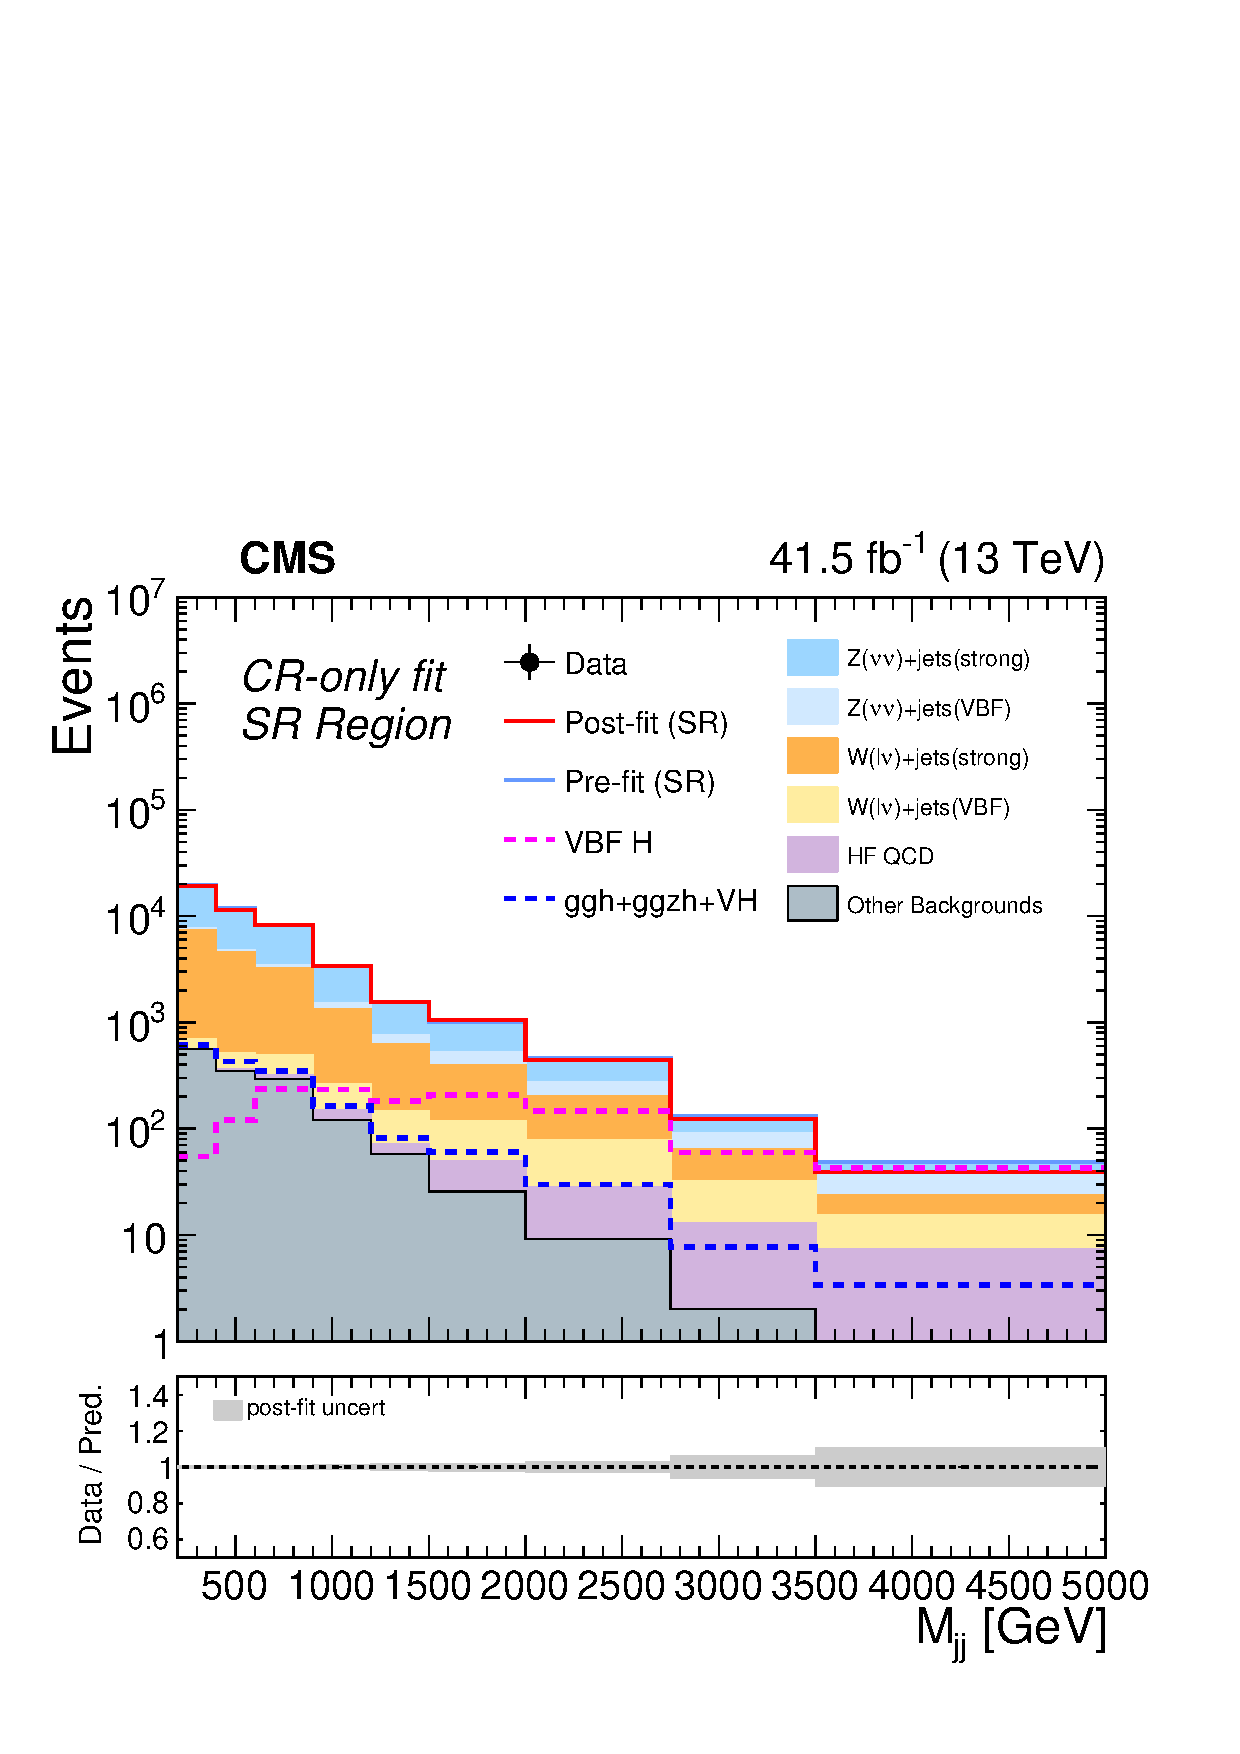
\includegraphics[width=0.45\textwidth]{\resultPlotDir/combined/vbf_2017_PULLS_MASKED_prefit_postfit_signal_2017.pdf}
        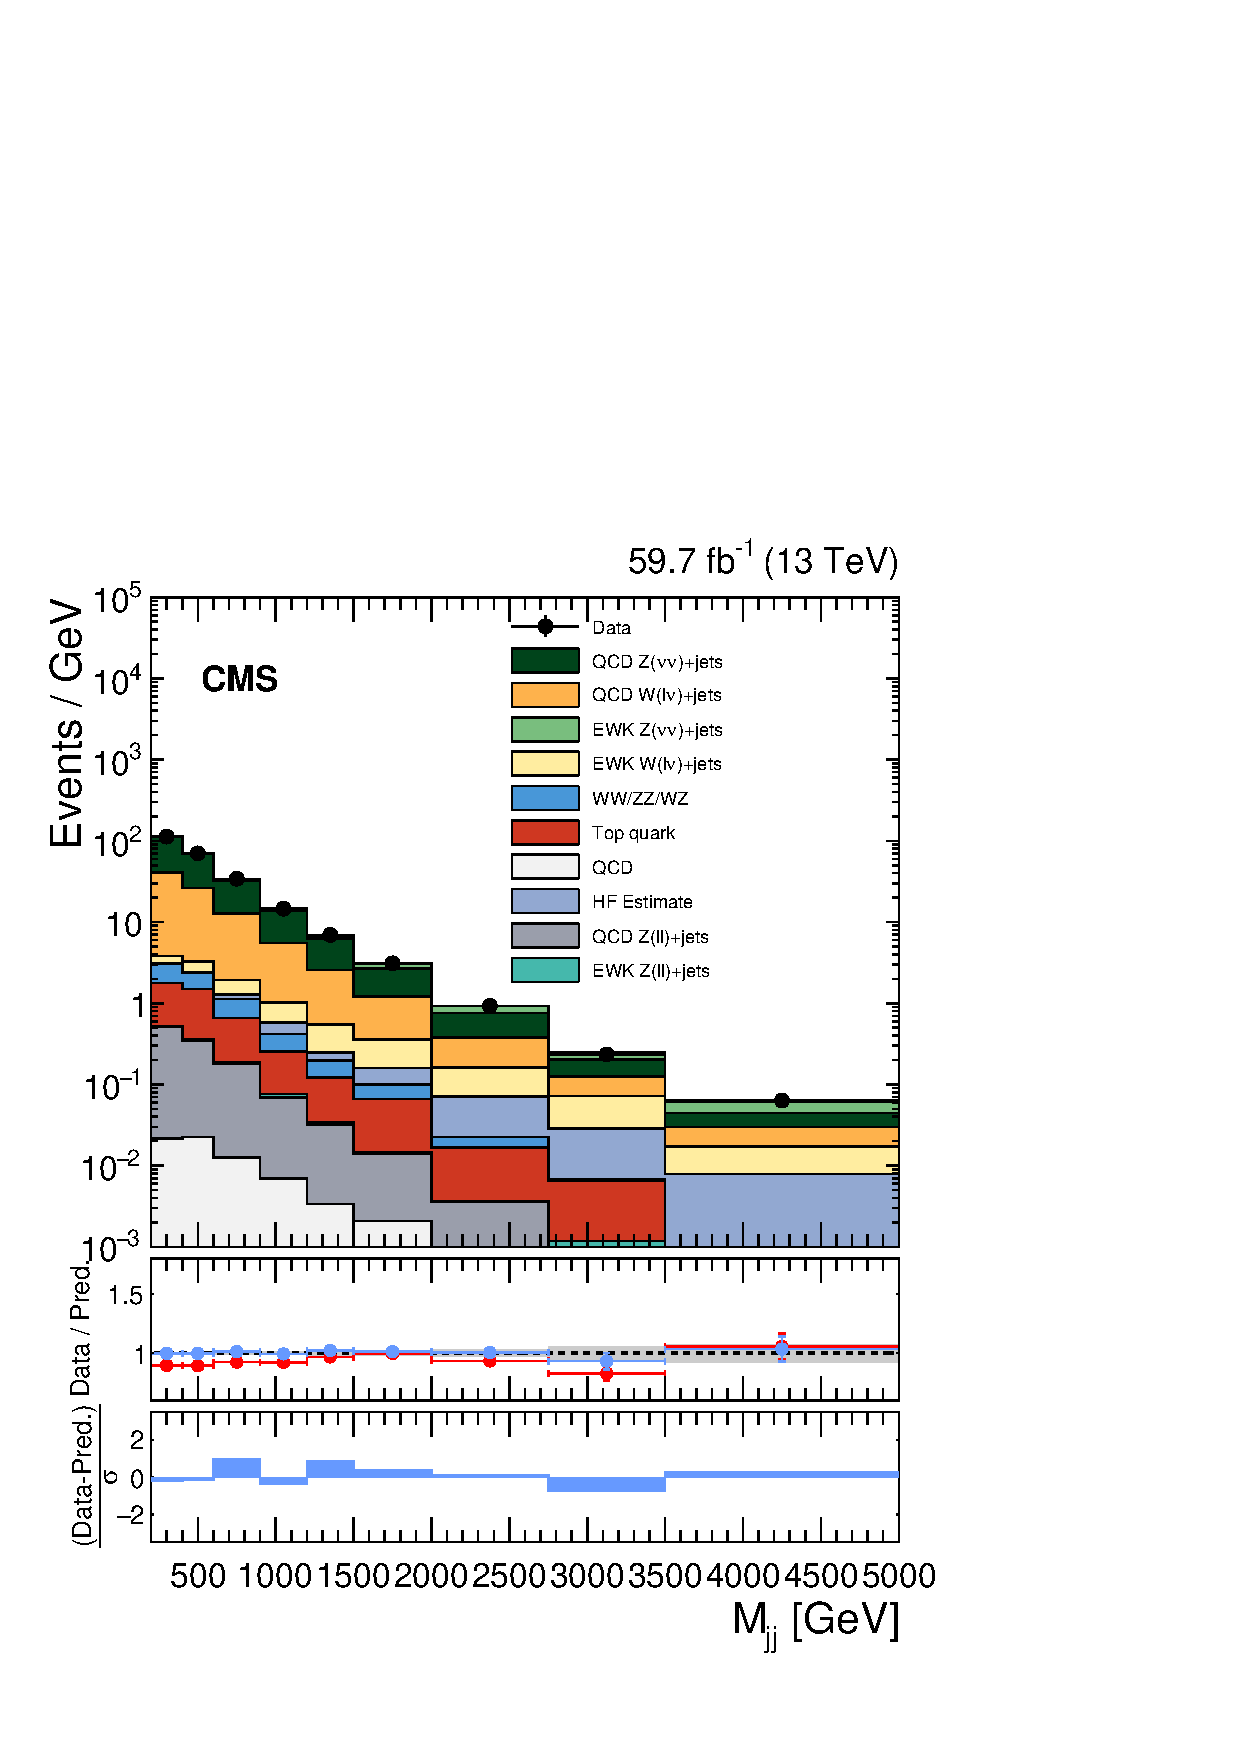
\includegraphics[width=0.45\textwidth]{\resultPlotDir/combined/vbf_2018_PULLS_MASKED_prefit_postfit_signal_2018.pdf} \\
        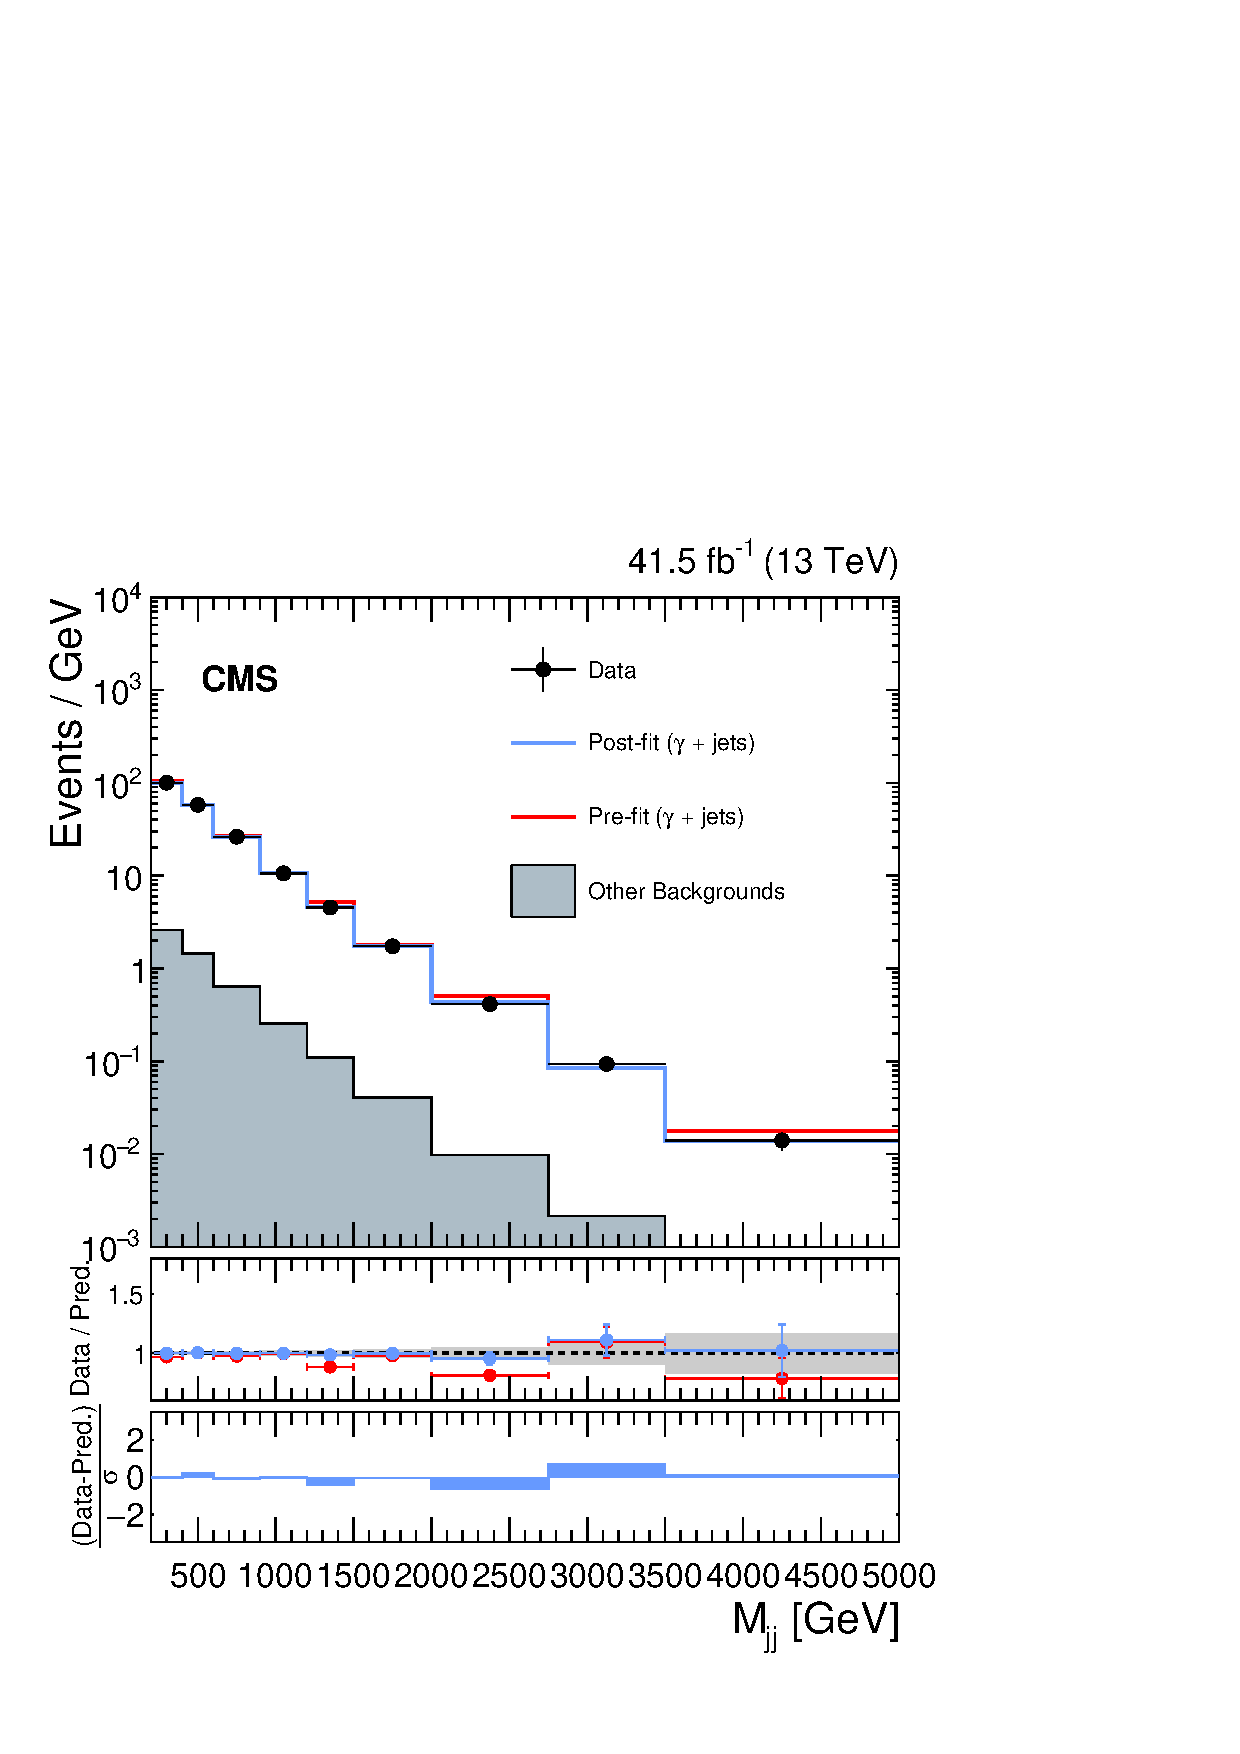
\includegraphics[width=0.45\textwidth]{\resultPlotDir/combined/vbf_2017_PULLS_MASKED_prefit_postfit_gjets_2017.pdf}
        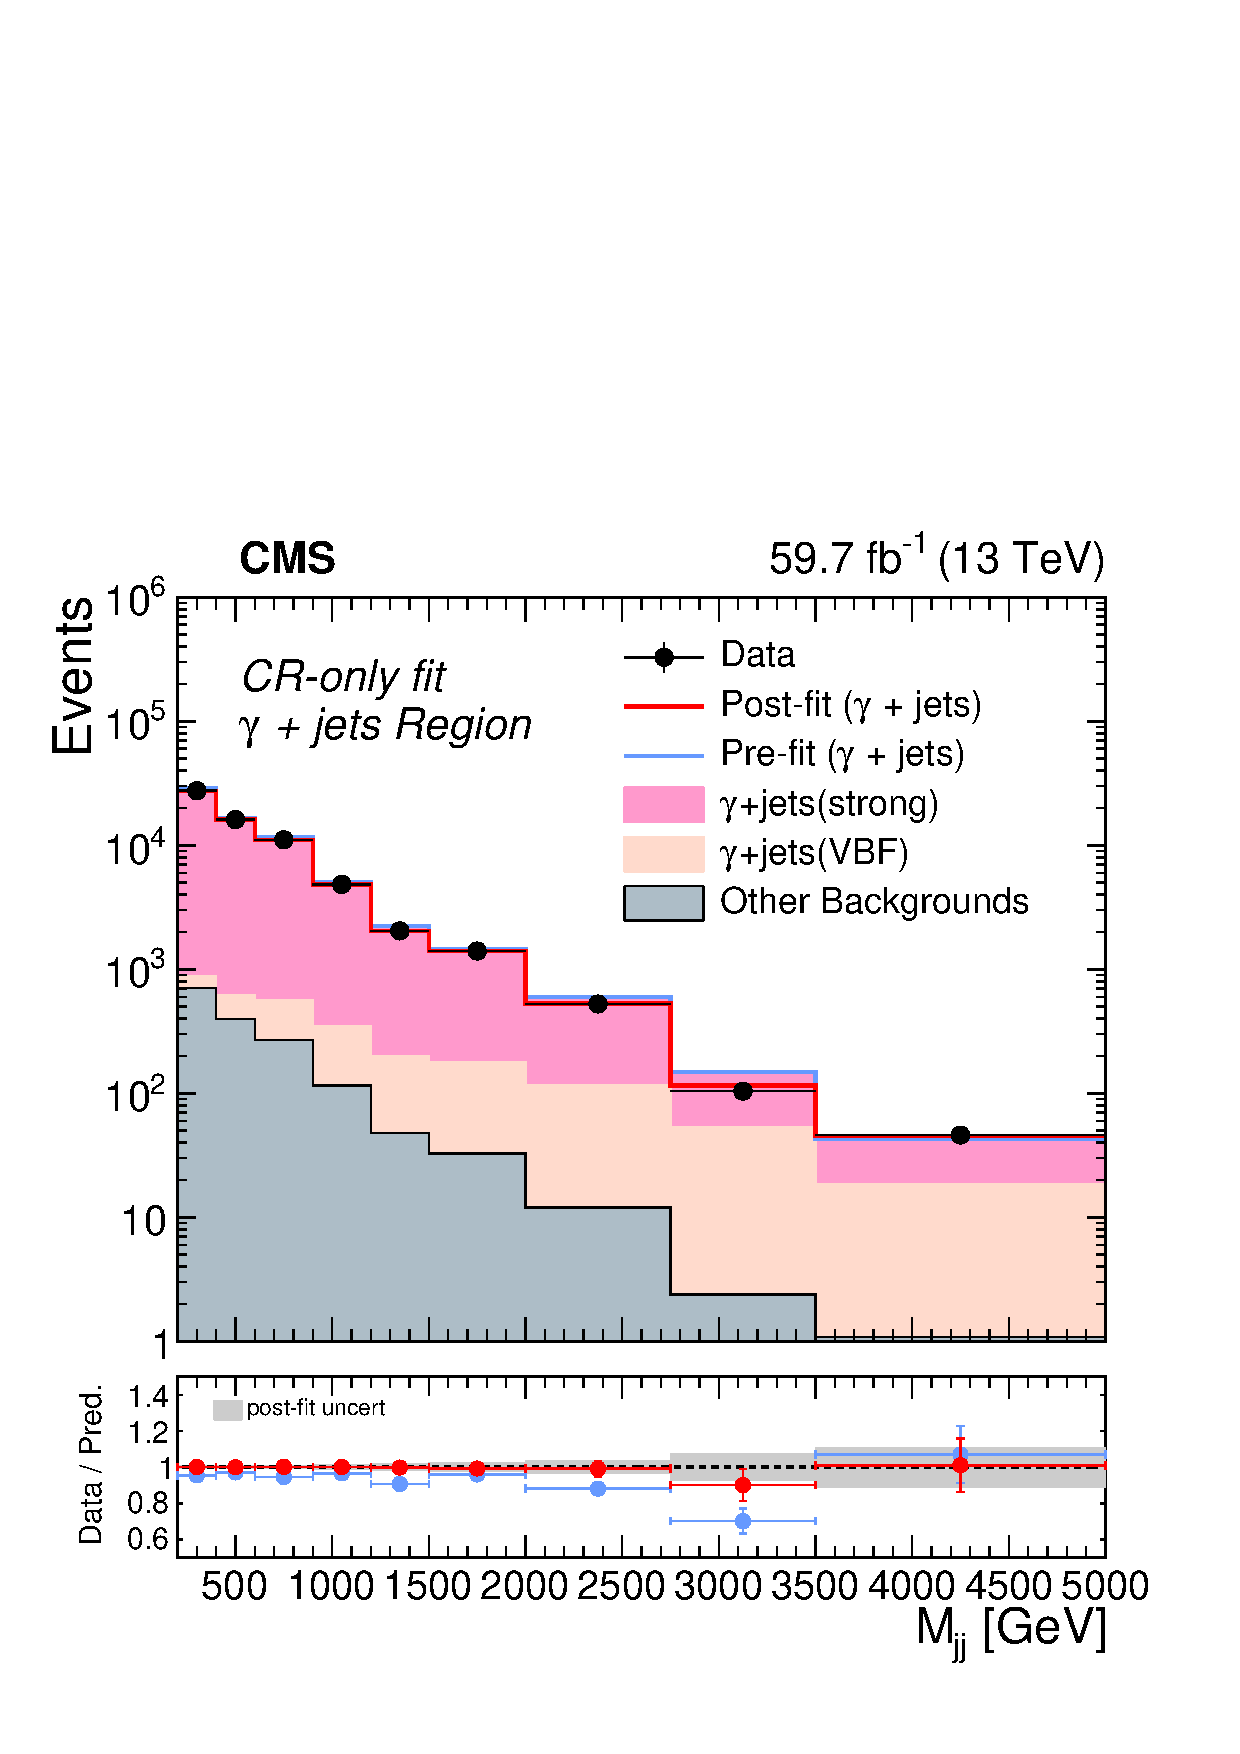
\includegraphics[width=0.45\textwidth]{\resultPlotDir/combined/vbf_2018_PULLS_MASKED_prefit_postfit_gjets_2018.pdf}
    \caption{Comparison between data and background estimation in VBF SR (top) and $\gamma$ + jets CR (bottom),
    before and after the simultaneous fit. The fit includes the data in all CRs and the signal region. The resulting
    distributions are shown separately for 2017 (left) and 2018 (right). In the ratio pads, ratios of data and background
    estimation are shown before (red) and after (blue) the fit. The gray band indicates the post-fit uncertainty.
    Finally, the distribution of the difference between data and post-fit background prediction relative to the quadrature sum of
    the uncertainties in the prediction and in data is shown in the lowest panel.}
    \label{fig:pre_postfit_sr_and_gamma}
\end{figure}

\begin{figure}[htbp]
    \centering
        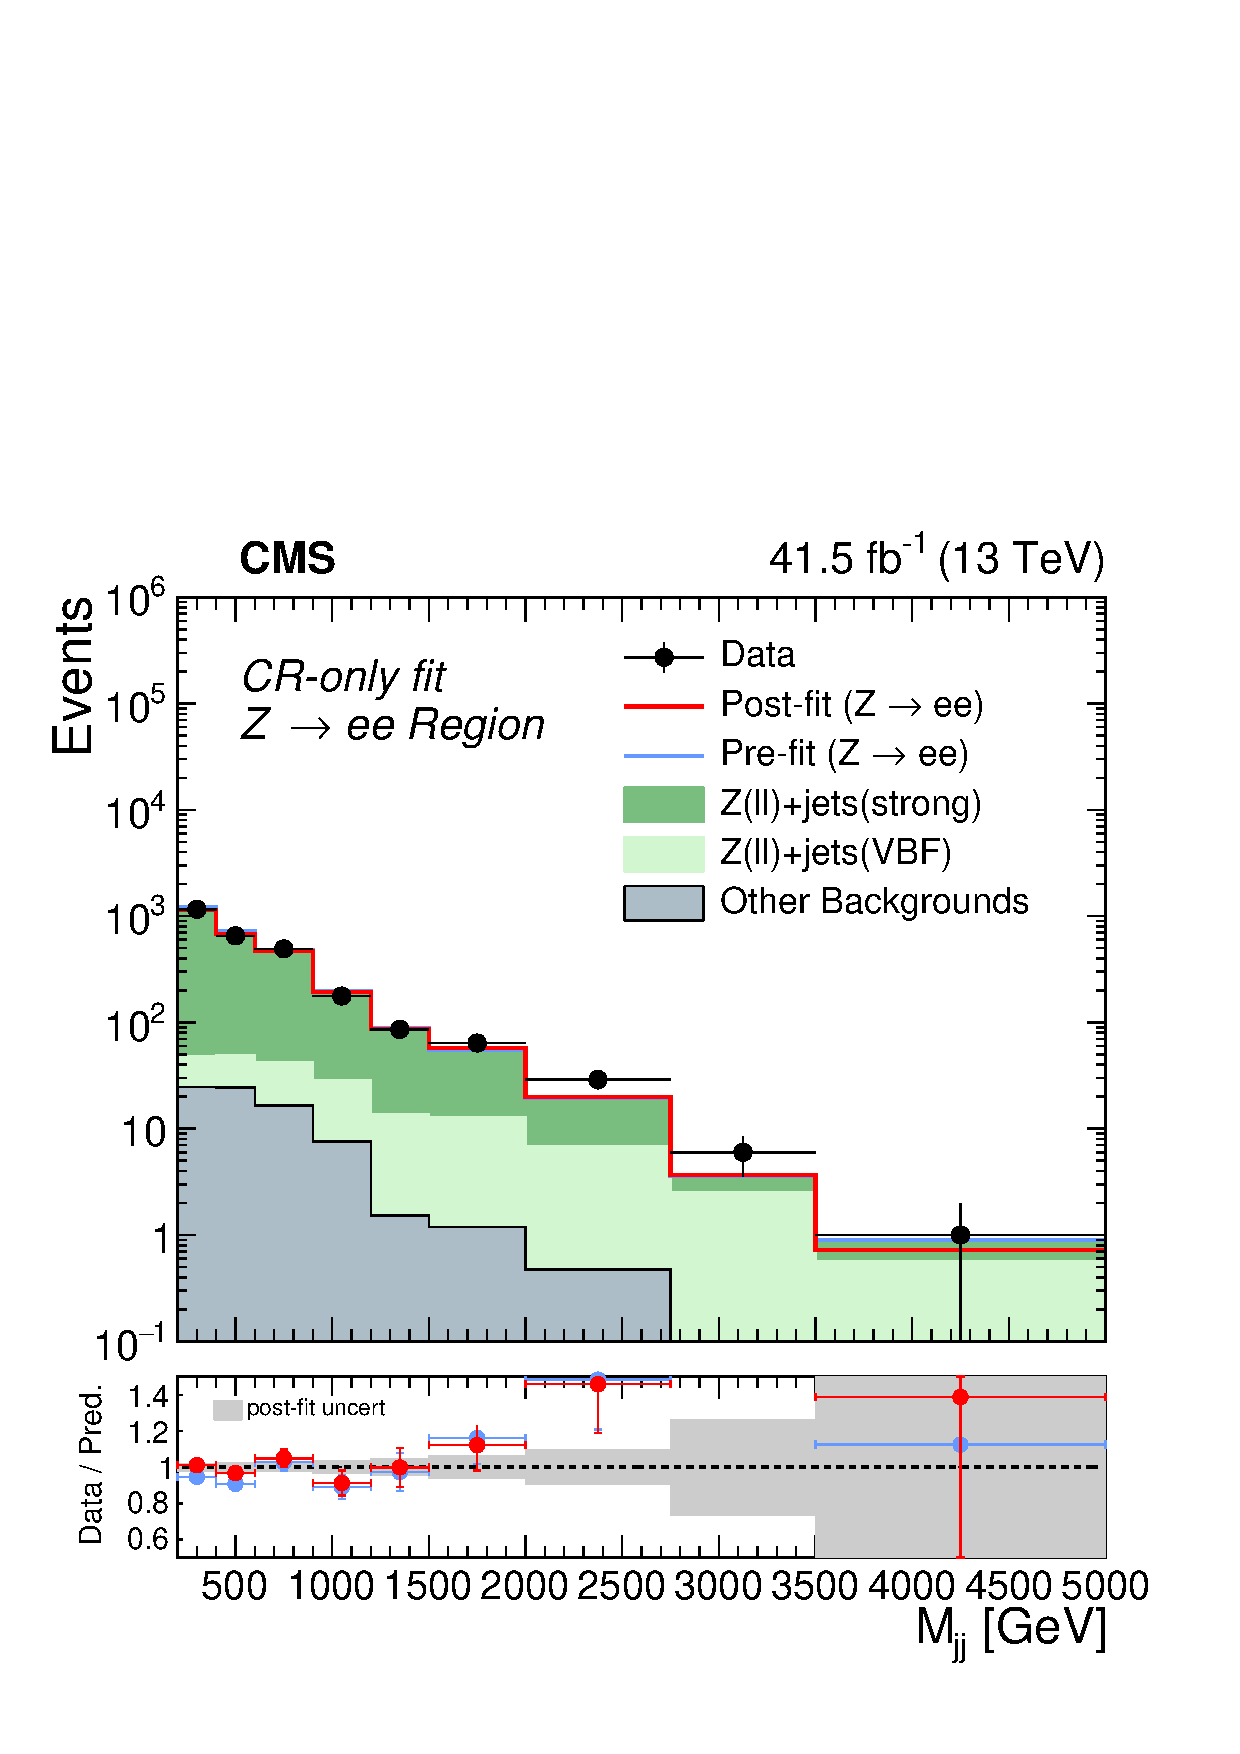
\includegraphics[width=0.45\textwidth]{\resultPlotDir/combined/vbf_2017_PULLS_MASKED_prefit_postfit_dielectron_2017.pdf}
        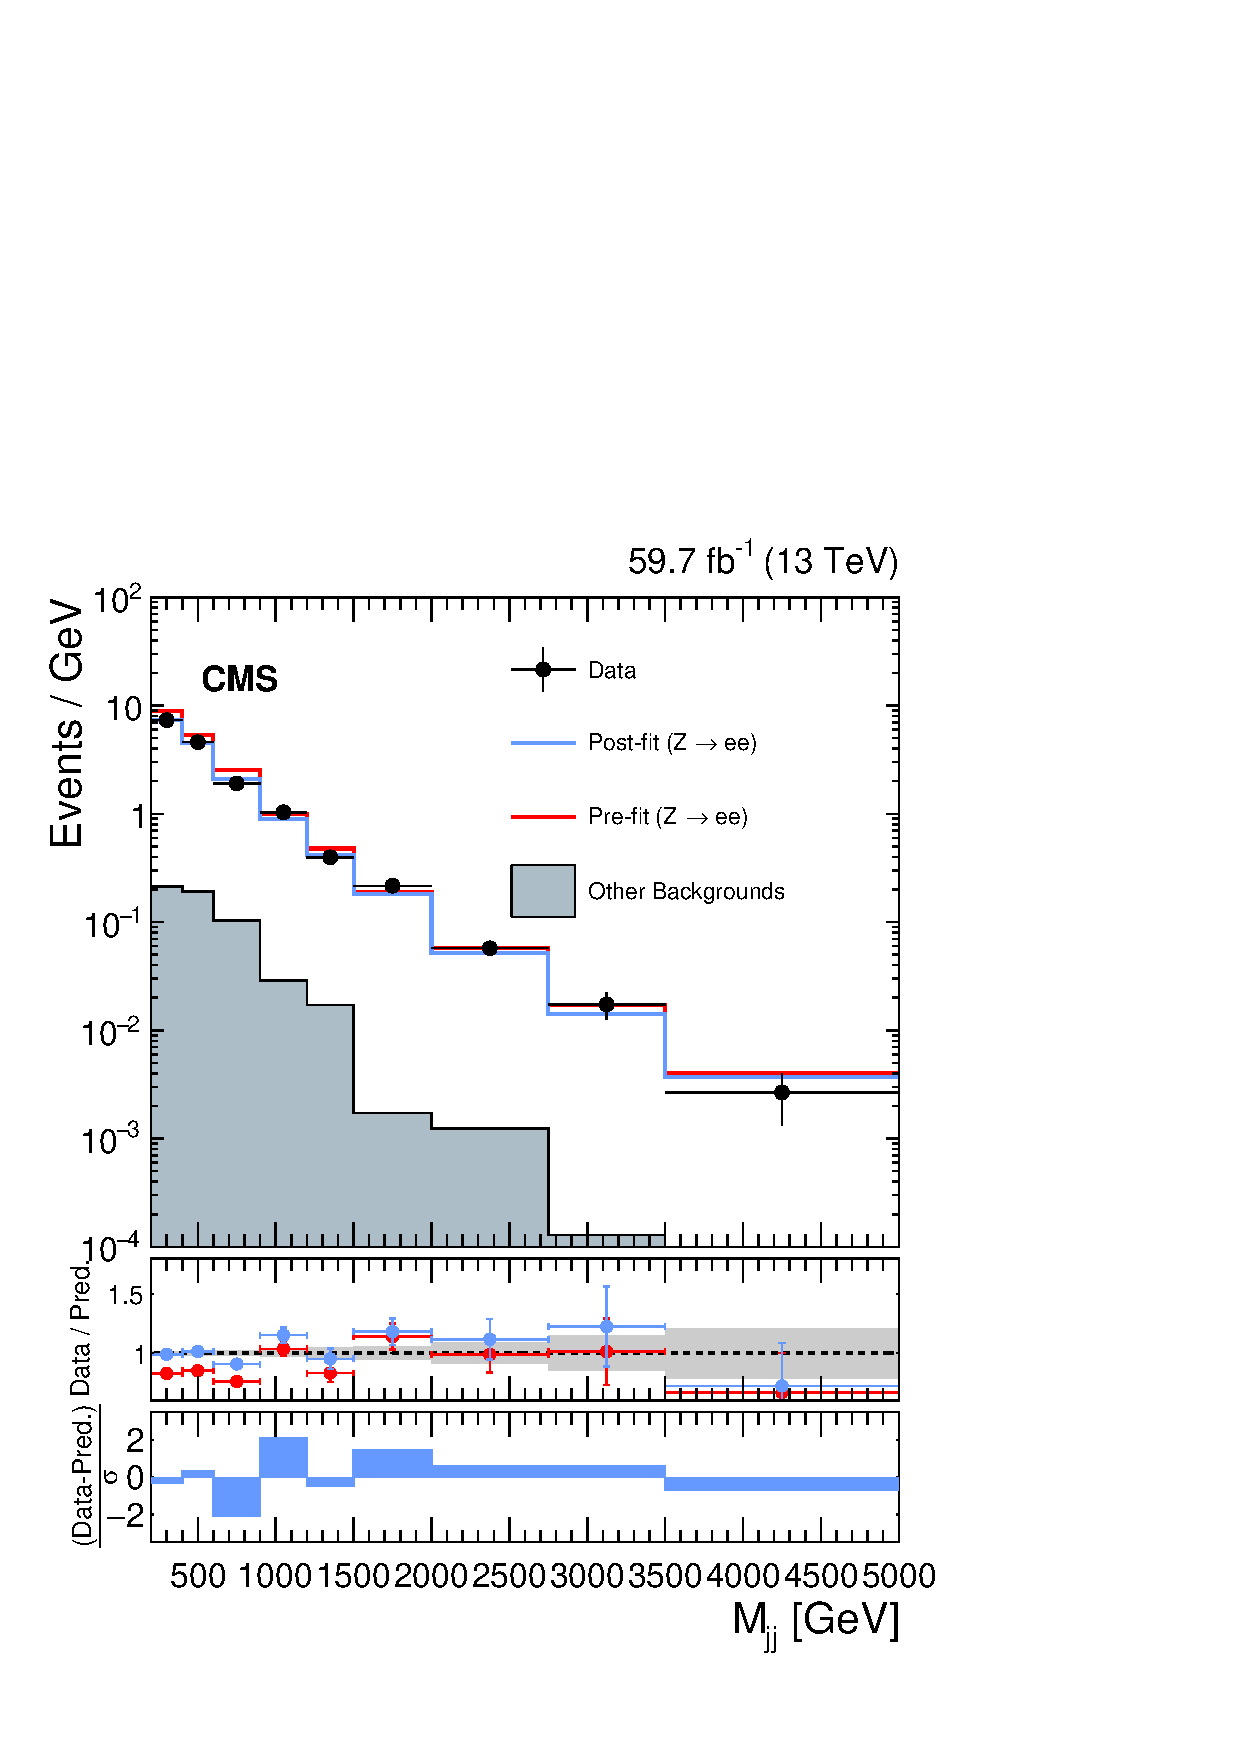
\includegraphics[width=0.45\textwidth]{\resultPlotDir/combined/vbf_2018_PULLS_MASKED_prefit_postfit_dielectron_2018.pdf} \\
        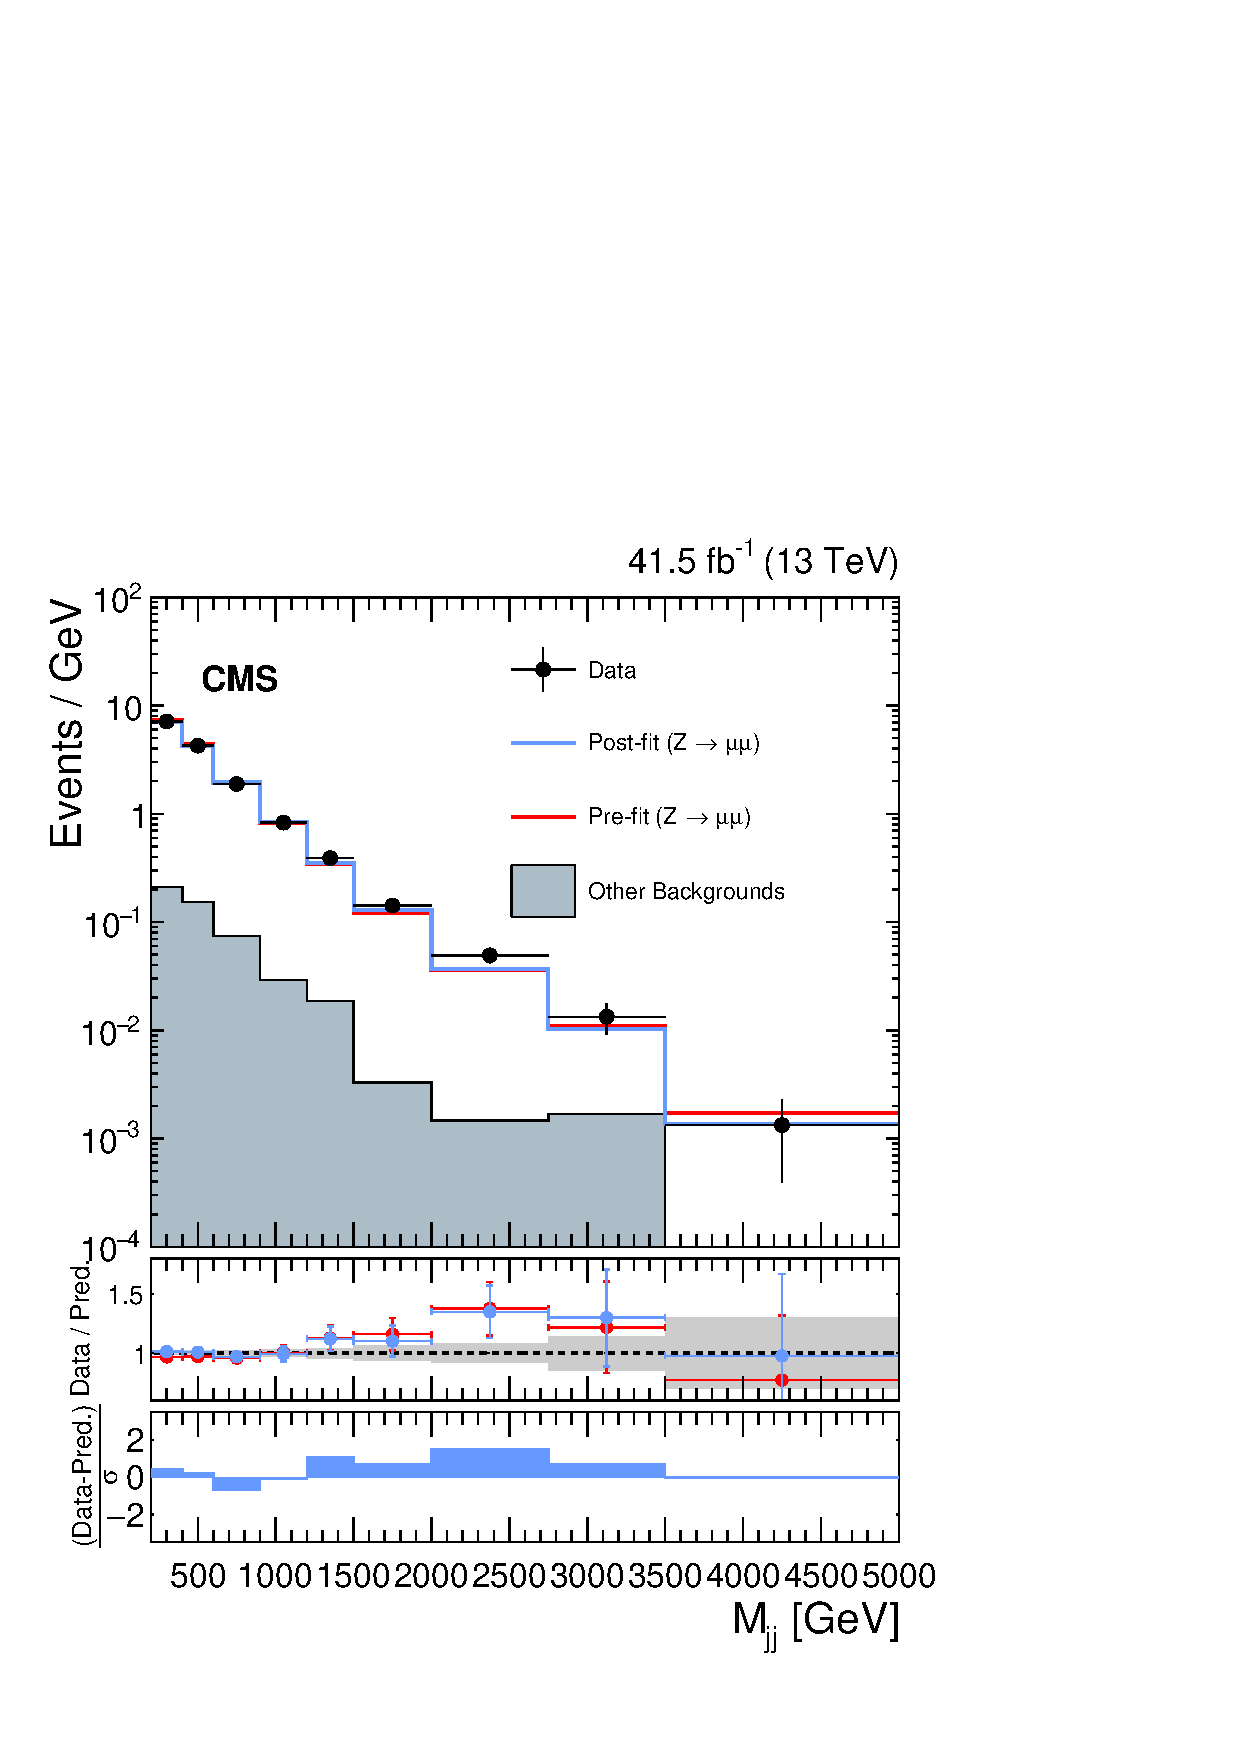
\includegraphics[width=0.45\textwidth]{\resultPlotDir/combined/vbf_2017_PULLS_MASKED_prefit_postfit_dimuon_2017.pdf}
        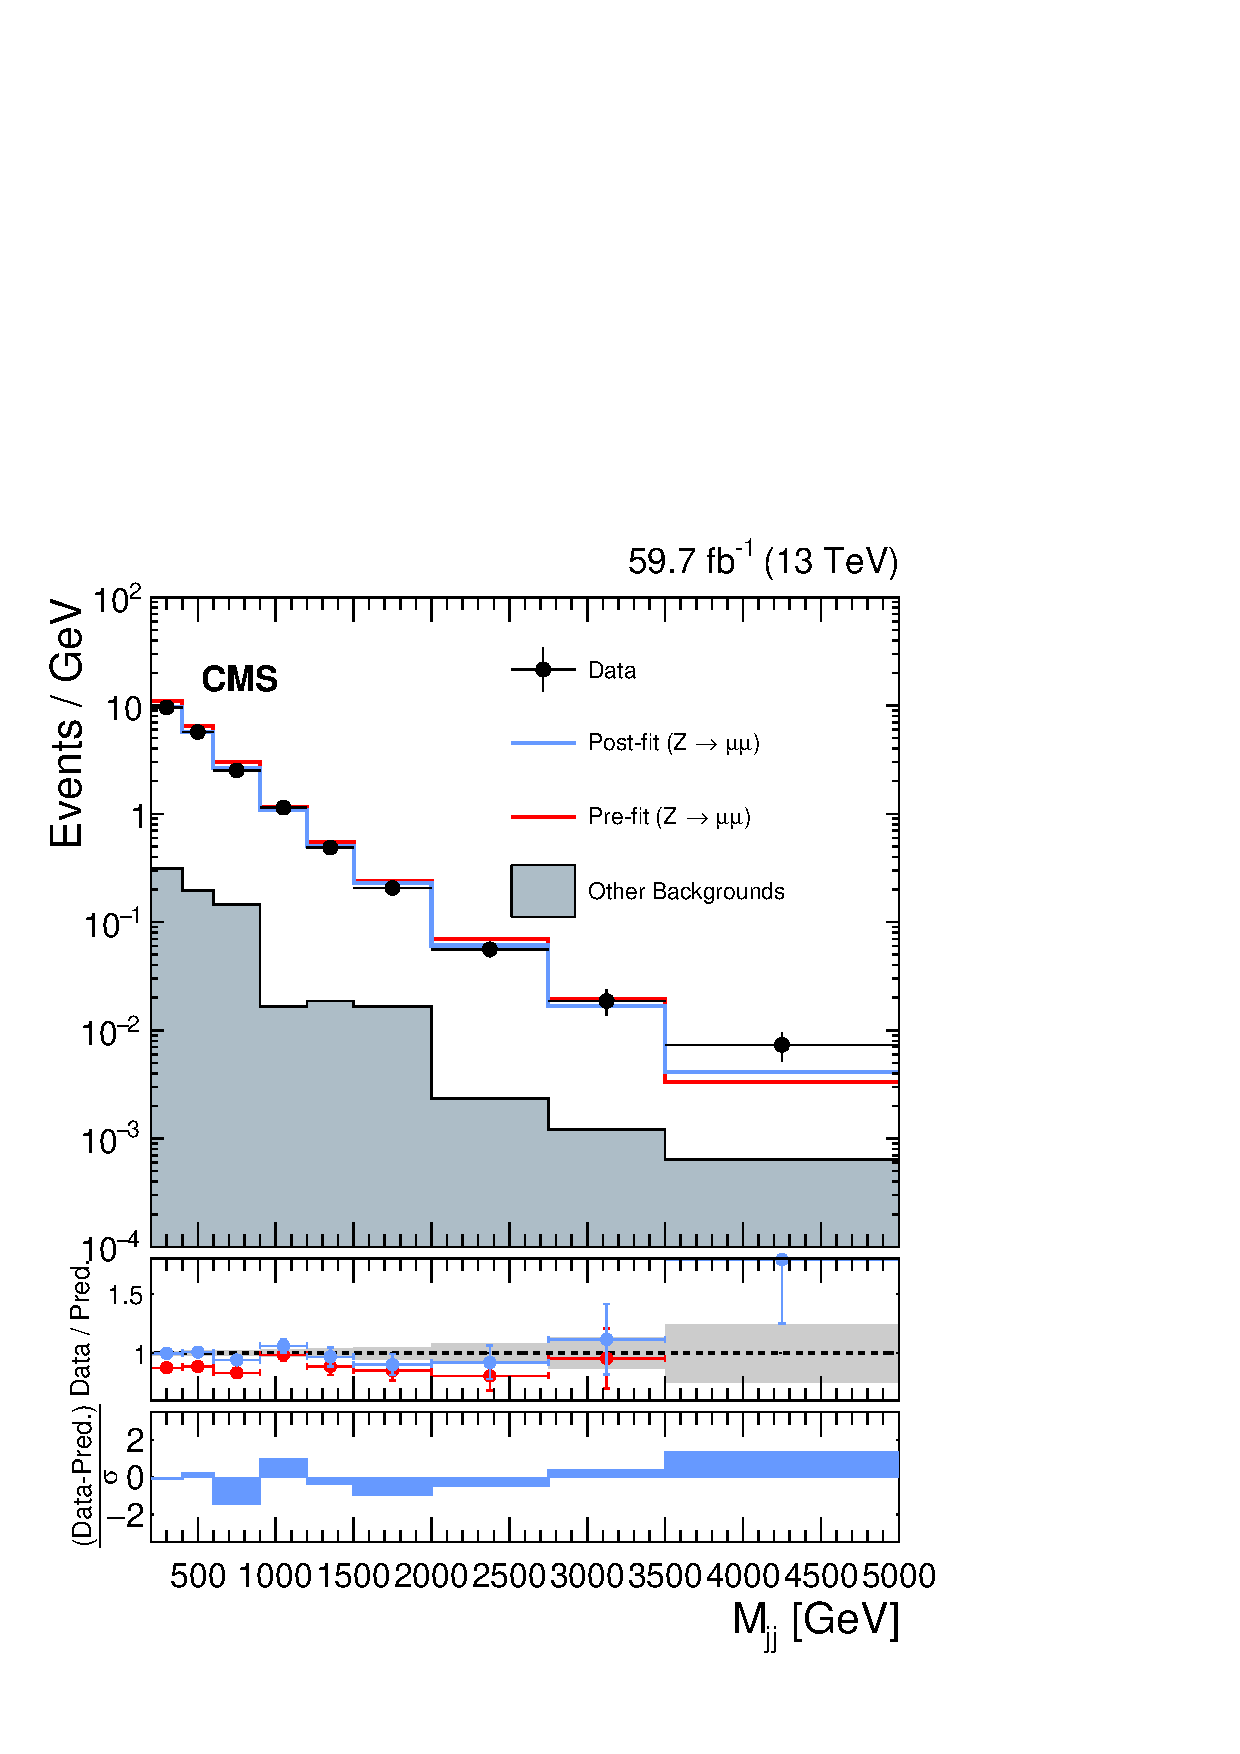
\includegraphics[width=0.45\textwidth]{\resultPlotDir/combined/vbf_2018_PULLS_MASKED_prefit_postfit_dimuon_2018.pdf}
    \caption{Same as Fig.~\ref{fig:pre_postfit_sr_and_gamma} but with dilepton CRs. The other backgrounds include top 
    quark and diboson processes.}
    \label{fig:pre_postfit_dilepton_regions}
\end{figure}

\begin{figure}[htbp]
    \centering
        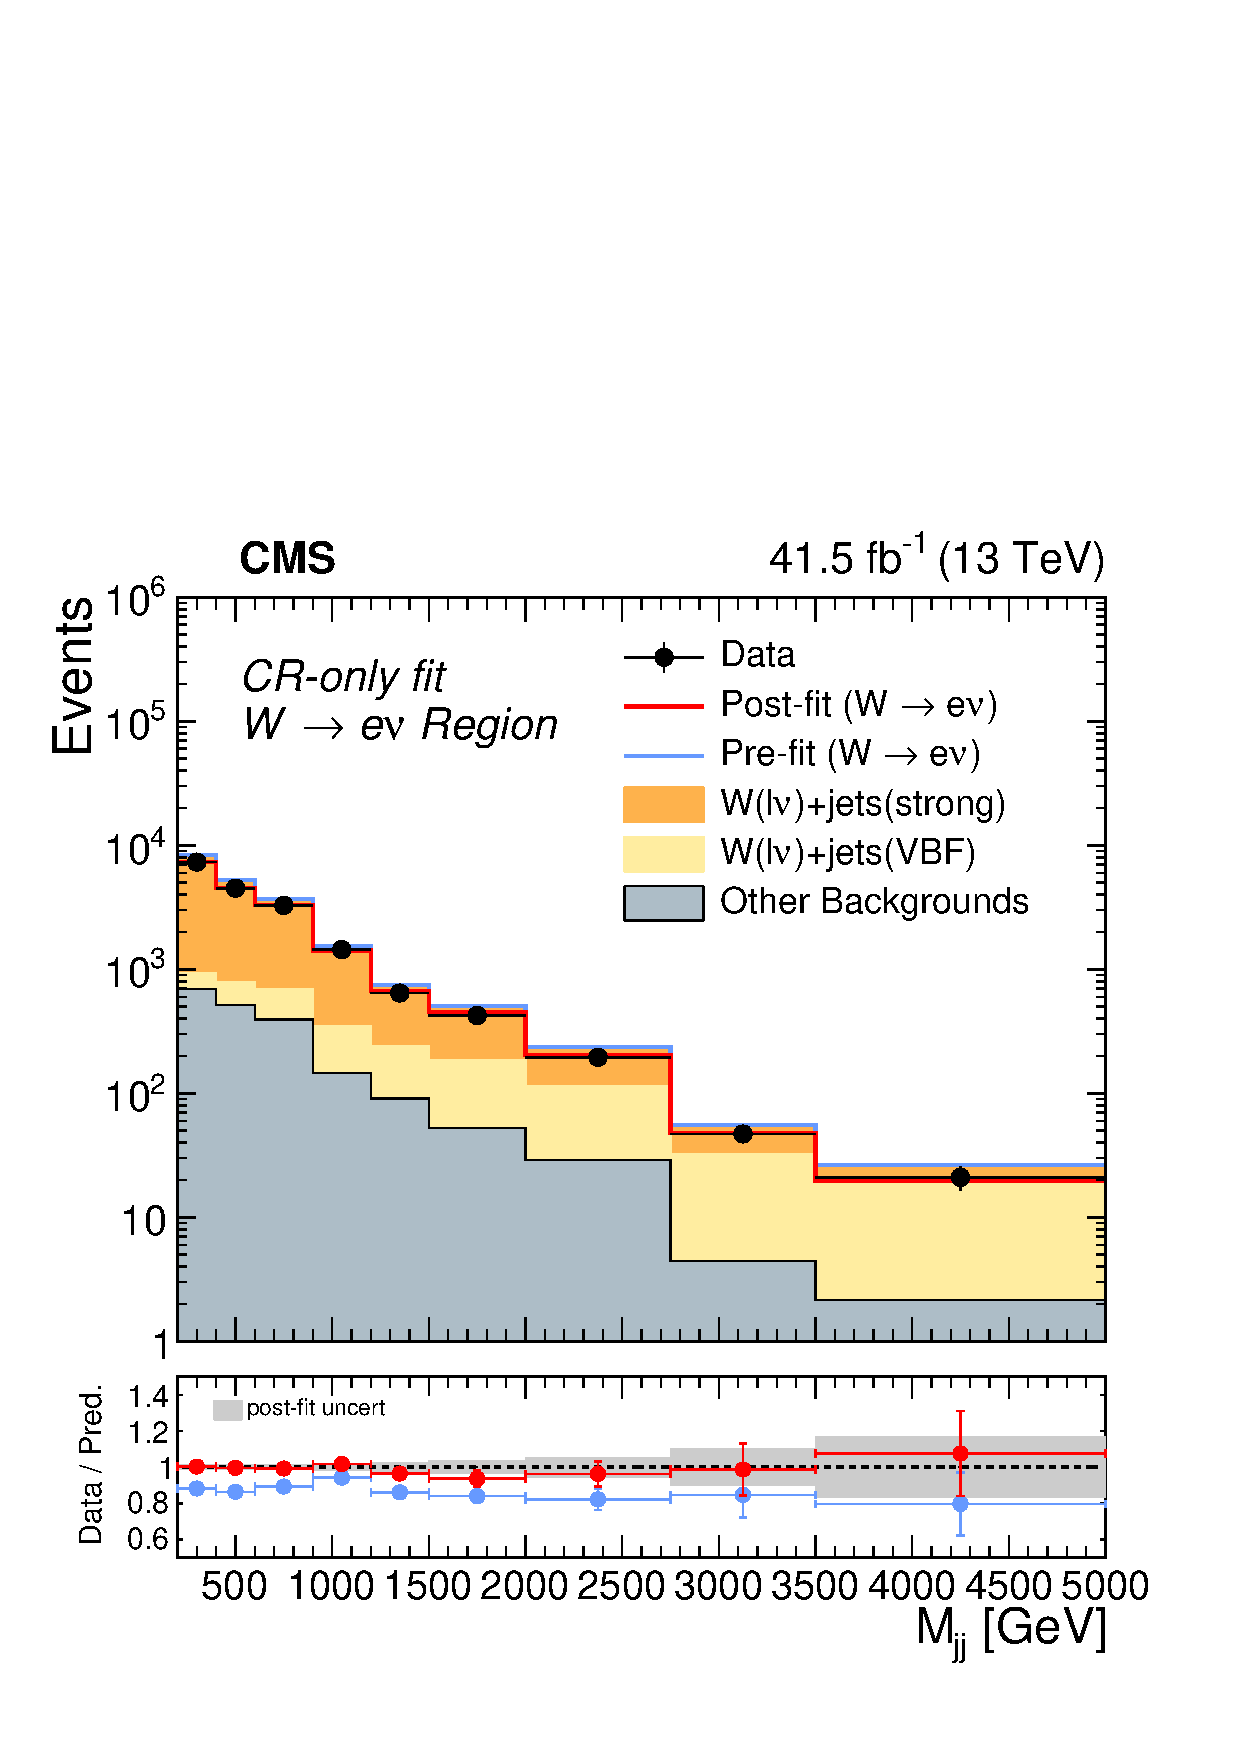
\includegraphics[width=0.45\textwidth]{\resultPlotDir/combined/vbf_2017_PULLS_MASKED_prefit_postfit_singleelectron_2017.pdf}
        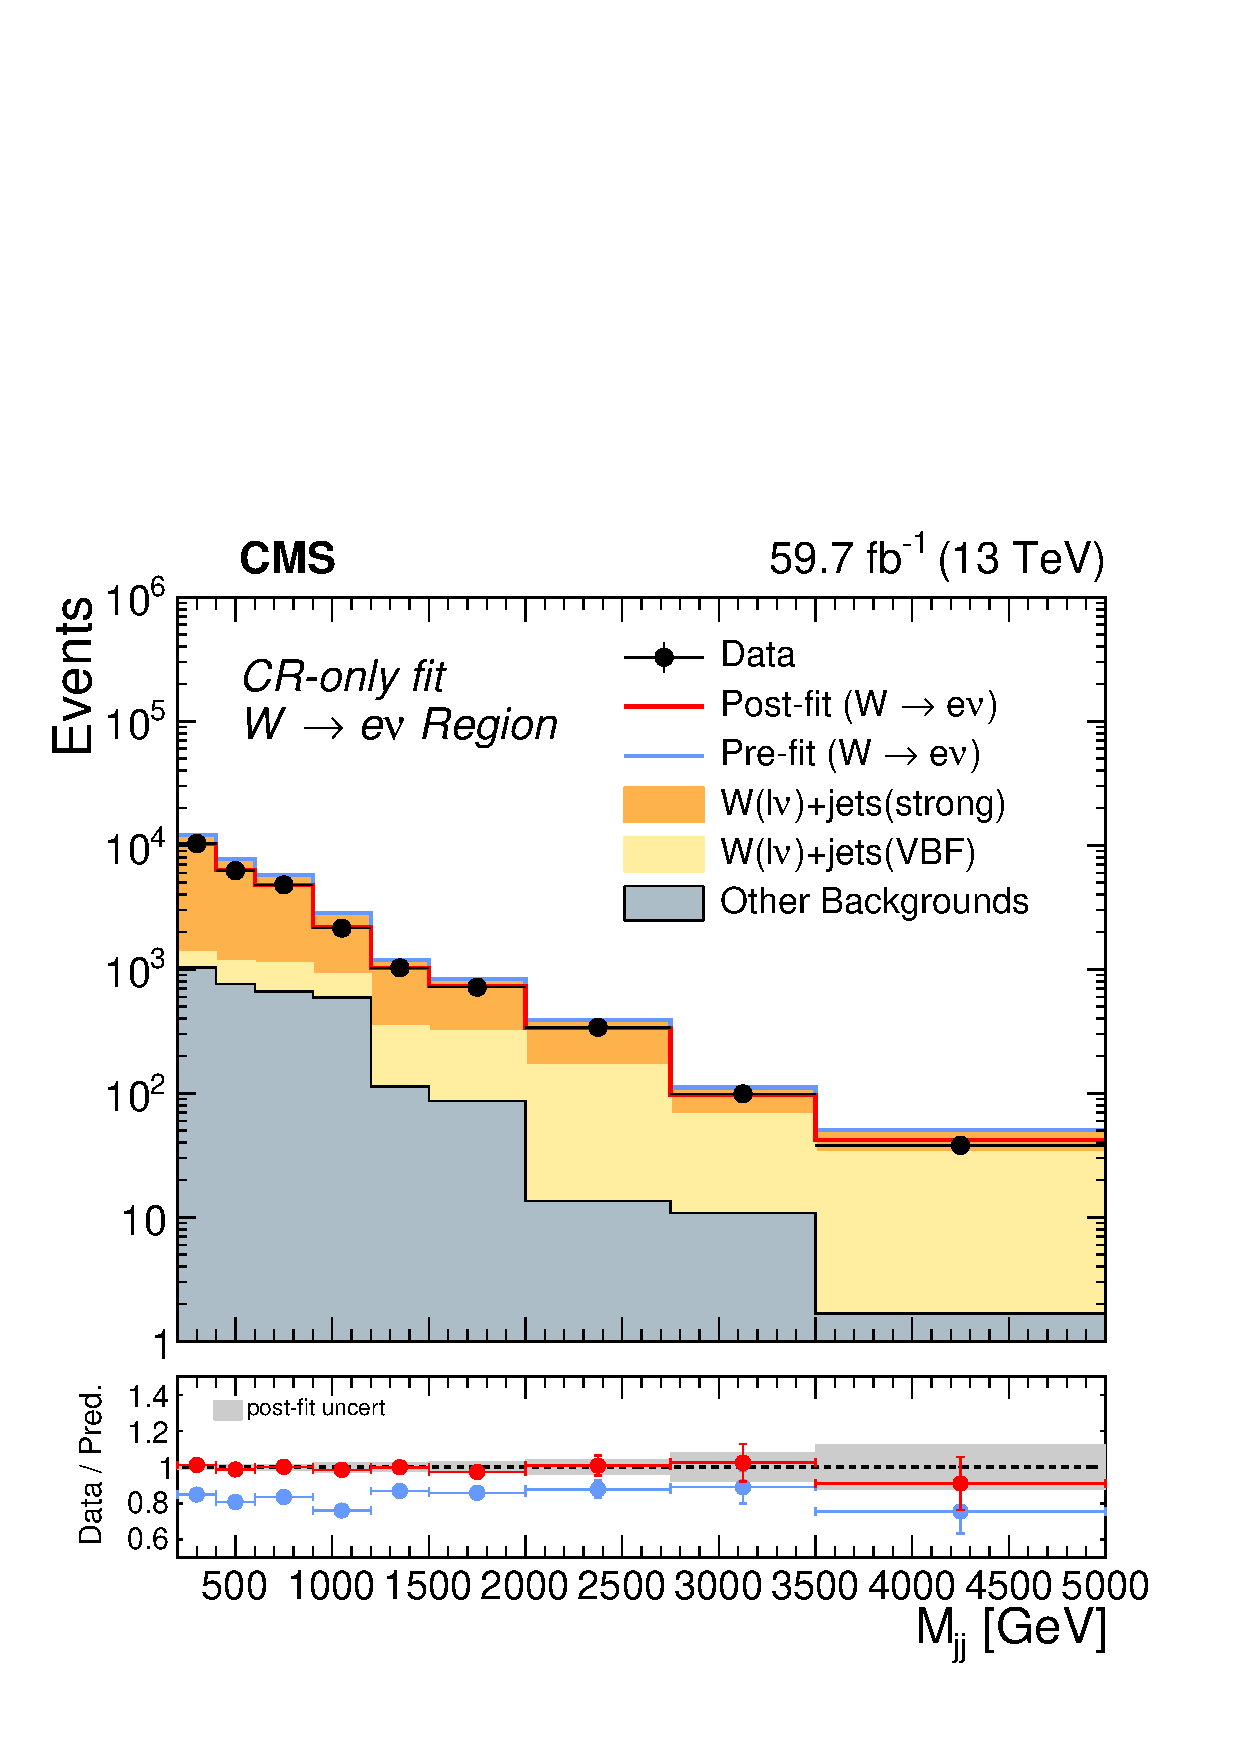
\includegraphics[width=0.45\textwidth]{\resultPlotDir/combined/vbf_2018_PULLS_MASKED_prefit_postfit_singleelectron_2018.pdf} \\
        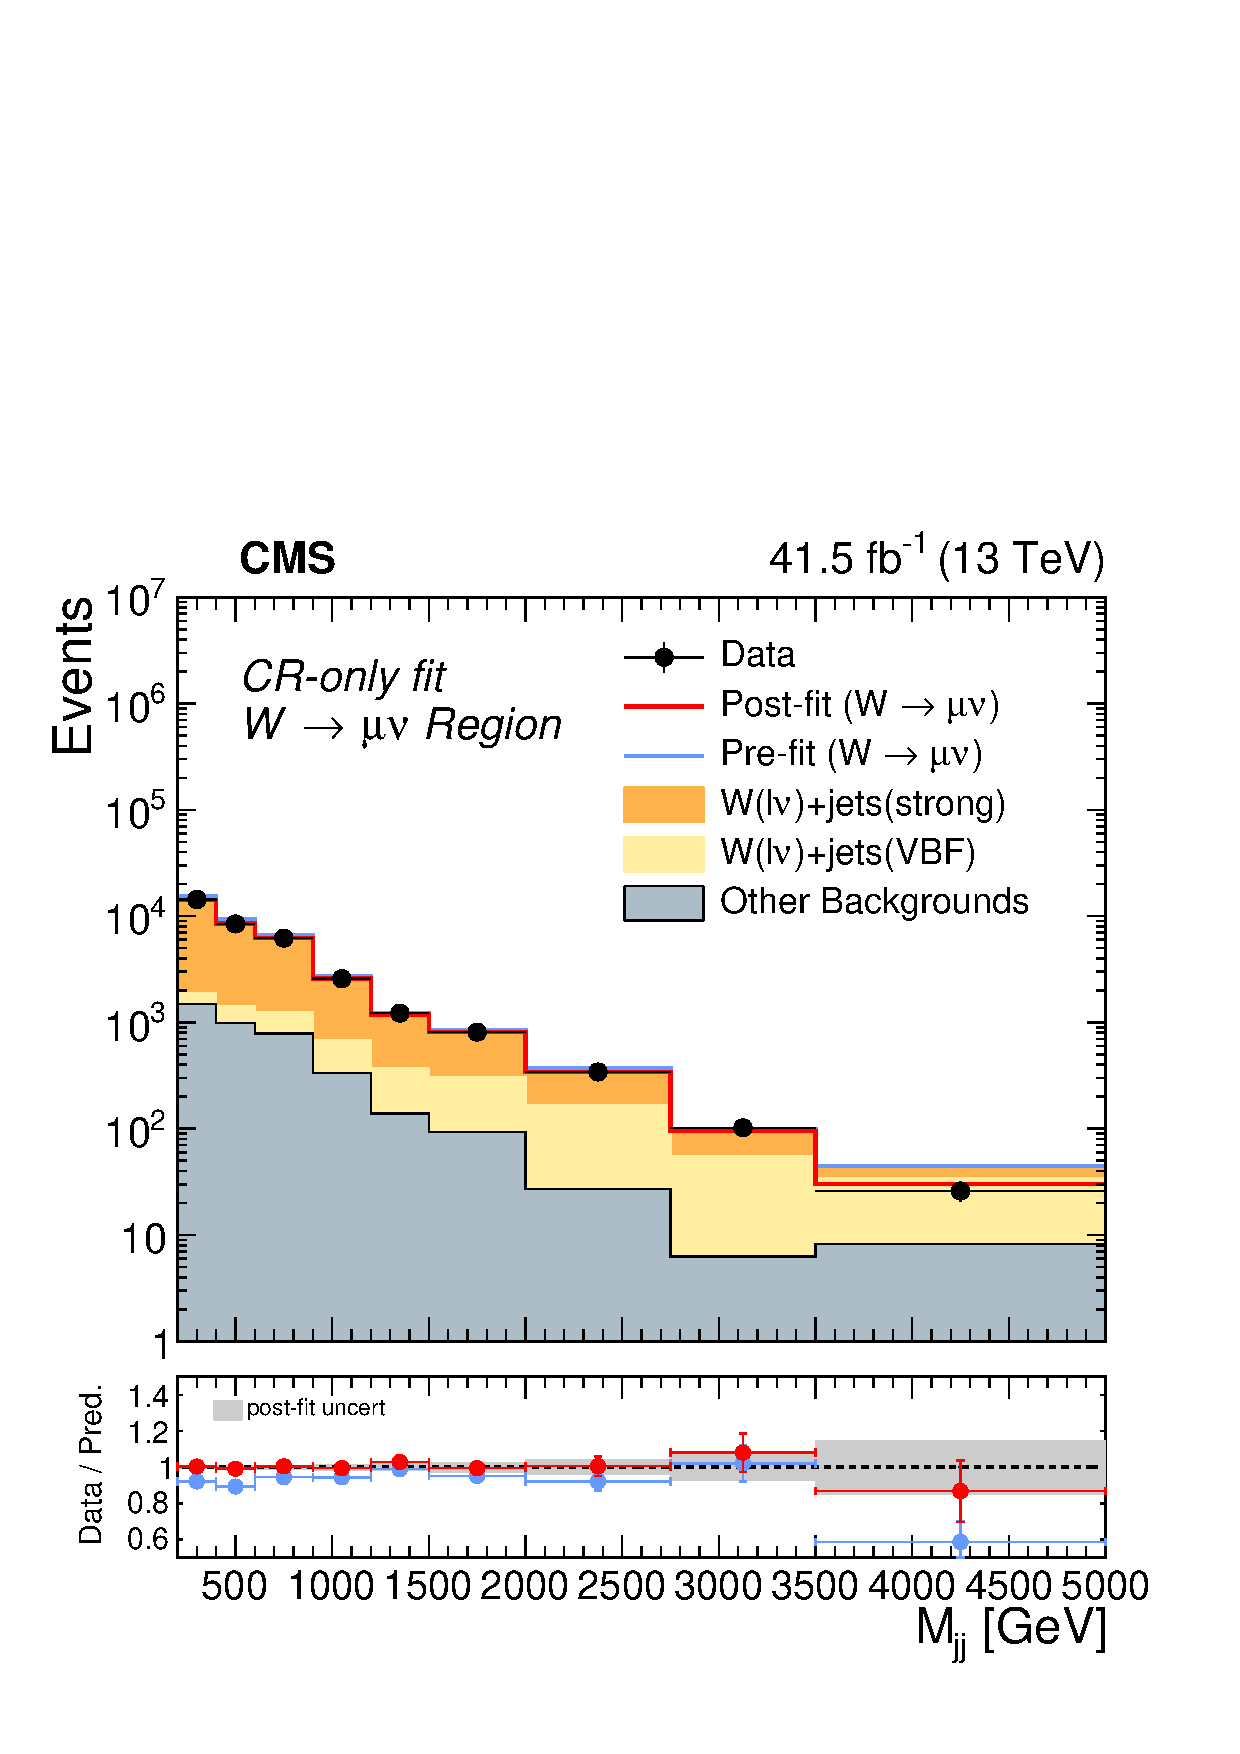
\includegraphics[width=0.45\textwidth]{\resultPlotDir/combined/vbf_2017_PULLS_MASKED_prefit_postfit_singlemuon_2017.pdf}
        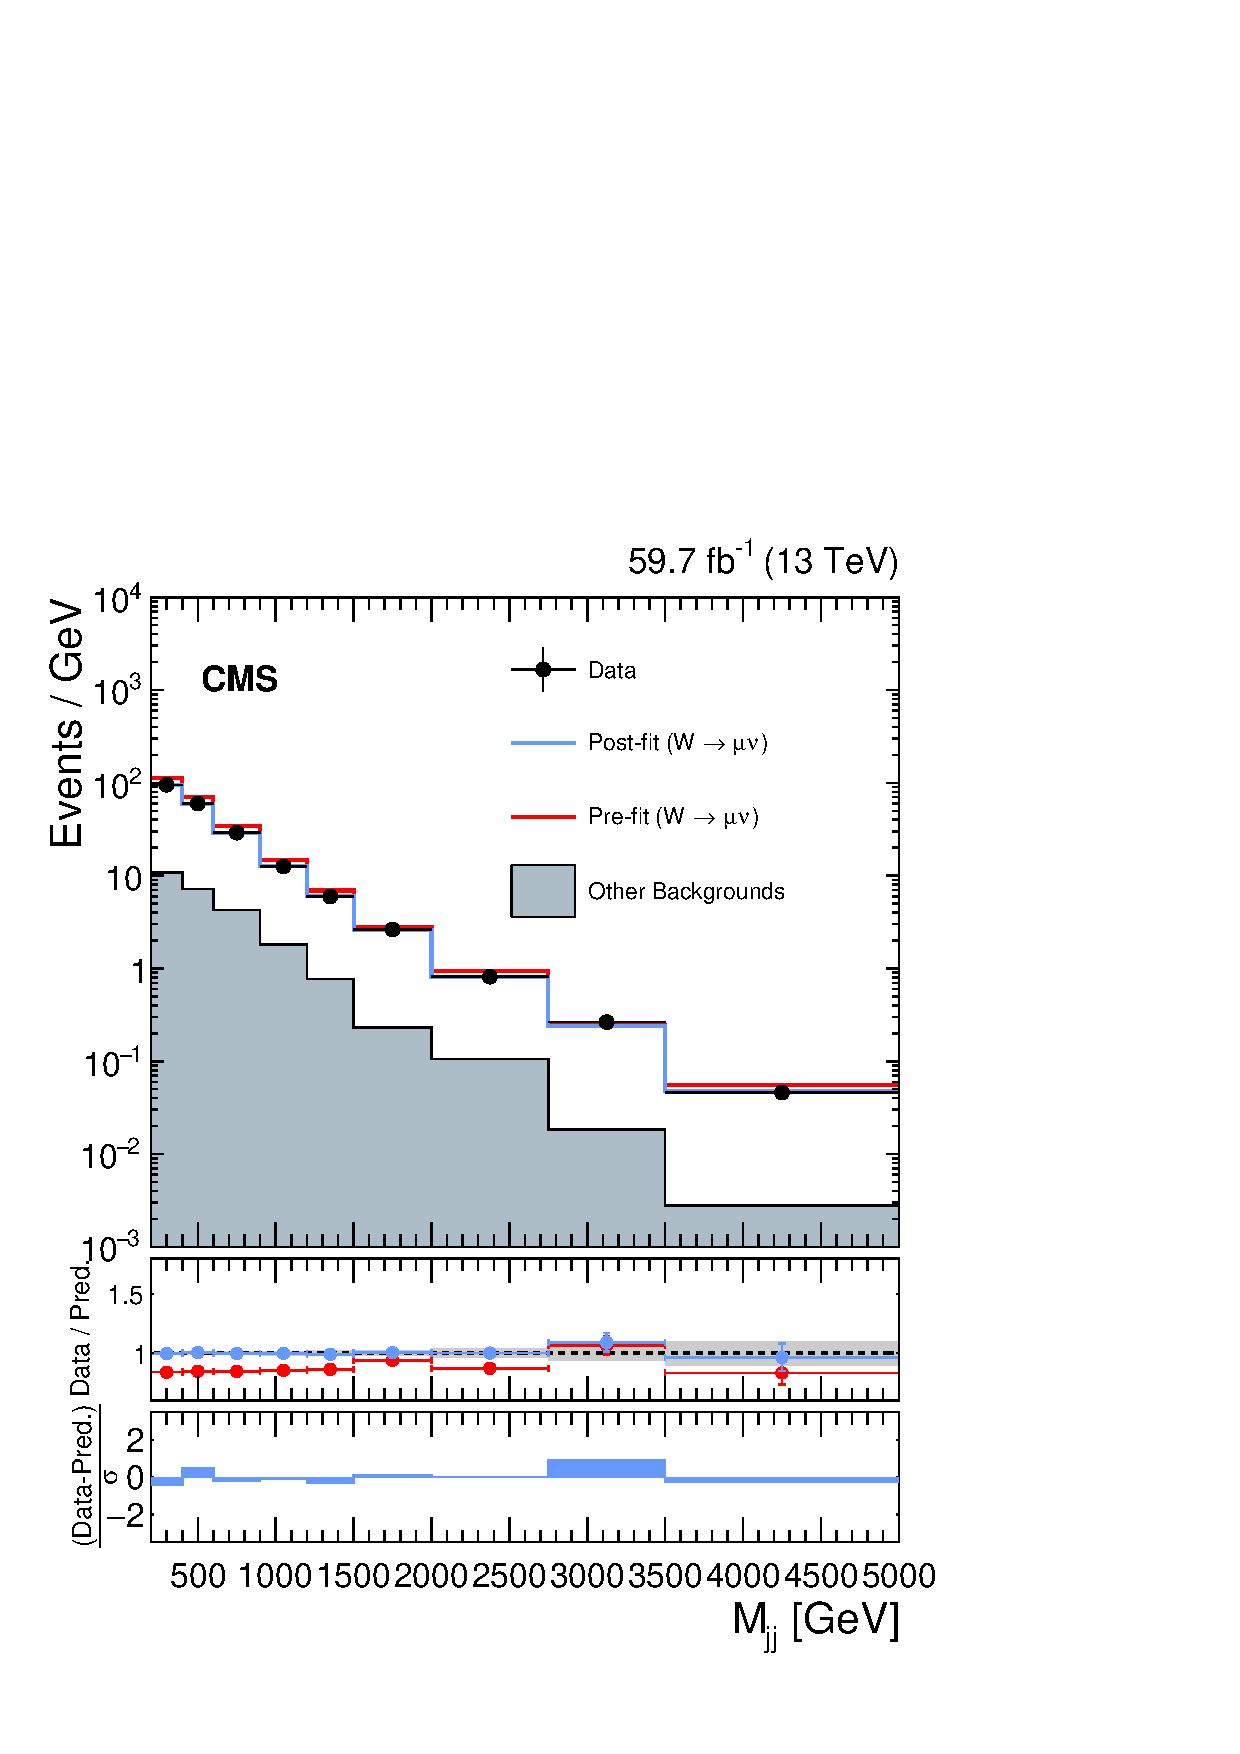
\includegraphics[width=0.45\textwidth]{\resultPlotDir/combined/vbf_2018_PULLS_MASKED_prefit_postfit_singlemuon_2018.pdf}
    \caption{Same as Fig.~\ref{fig:pre_postfit_sr_and_gamma} but with single lepton CRs. The other backgrounds include top 
    quark and diboson processes.}
    \label{fig:pre_postfit_single_lepton_regions}
\end{figure}

\clearpage

\begin{sidewaystable}[h!]
    \centering
    \caption{
        Expected event yields in each $\mjj$ bin for the different background
        processes in the VBF signal region, with the 2017 samples. The
        background yields and the corresponding uncertainties are obtained
        after performing a combined fit across all of the CRs and SR. The
        expected signal contributions for a Higgs boson, produced in the non-VBF
        and VBF modes, decaying to invisible particles with a branching
        fraction of $\brinv = 1$, and the observed event yields are also
        reported.}
        \cmsTable{
            \renewcommand{\arraystretch}{1.2}
            \begin{tabular}{l|c|c|c|c|c|c|c|c|c}
\mjj bin range (\GeV) & 200-400 & 400-600 & 600-900 & 900-1200 & 1200-1500 & 1500-2000 & 2000-2750 & 2750-3500 & $>$3500  \\
\hline
\hline
$Z(\nu\nu)+\textrm{jets}$ (strong)  & $11957.1\pm55.5$ & $7022.4\pm42.2$ & $4855.8\pm34.6$ & $1914.1\pm17.6$ & $826.8\pm11.4$ & $531.3\pm8.5$ & $183.5\pm4.7$ & $39.6\pm4.1$ & $8.3\pm0.9$\\
$Z(\nu\nu)+\textrm{jets}$ (VBF)  & $202.5\pm4.1$ & $222.2\pm4.1$ & $272.3\pm4.3$ & $197.6\pm3.8$ & $127.2\pm3.2$ & $126.4\pm3.6$ & $74.0\pm2.9$ & $25.3\pm2.9$ & $11.5\pm1.4$\\
$W(\ell\nu)+\textrm{jets}$ (strong)  & $6247.9\pm57.1$ & $3727.1\pm36.6$ & $2624.7\pm31.6$ & $1052.3\pm15.7$ & $450.0\pm11.7$ & $285.5\pm7.1$ & $116.5\pm4.9$ & $27.1\pm2.7$ & $5.1\pm1.0$\\
$W(\ell\nu)+\textrm{jets}$ (VBF)  & $122.6\pm7.2$ & $137.9\pm7.5$ & $161.9\pm8.1$ & $109.4\pm5.3$ & $72.3\pm3.5$ & $65.8\pm3.1$ & $45.7\pm2.9$ & $17.5\pm1.8$ & $5.9\pm0.8$\\
$t\bar{t}$ + single-top  & $237.6\pm16.0$ & $135.8\pm9.1$ & $124.0\pm8.0$ & $60.1\pm3.7$ & $30.7\pm2.0$ & $9.7\pm0.8$ & $2.7\pm0.3$ & $0.9\pm0.2$ & $0.4\pm0.1$\\
Diboson  & $201.0\pm24.8$ & $132.9\pm16.0$ & $101.7\pm12.2$ & $34.4\pm4.2$ & $15.8\pm1.9$ & $9.2\pm1.2$ & $3.3\pm0.5$ & $0.3\pm0.0$ & $0.0\pm0.0$\\
$Z/\gamma^{*}(\ell^{+}\ell^{-})+\mathrm{jets}$  & $86.6\pm3.3$ & $54.9\pm2.1$ & $44.7\pm1.6$ & $15.7\pm0.6$ & $6.0\pm0.4$ & $4.3\pm0.3$ & $2.6\pm0.2$ & $0.5\pm0.1$ & $0.1\pm0.0$\\
Multijet  & $6.6\pm1.5$ & $6.1\pm1.4$ & $6.6\pm1.5$ & $2.7\pm0.6$ & $1.3\pm0.3$ & $1.1\pm0.2$ & $0.4\pm0.1$ & $0.2\pm0.0$ & $0.1\pm0.0$\\
HF Noise  & $0.8\pm0.1$ & $16.6\pm2.1$ & $28.2\pm3.6$ & $25.1\pm3.2$ & $9.3\pm1.2$ & $18.4\pm2.3$ & $18.2\pm2.3$ & $10.7\pm1.4$ & $7.4\pm0.9$\\
$\mathrm{gg}H(\rightarrow \mathrm{inv.})$  & $570.5 $ & $411.5 $ & $338.0 $ & $162.8 $ & $82.5 $ & $61.8 $ & $30.4 $ & $8.1 $ & $3.6 $\\
$\mathrm{qq}H(\rightarrow \mathrm{inv.})$  & $56.2 $ & $125.7 $ & $245.8 $ & $244.0 $ & $191.2 $ & $217.9 $ & $156.1 $ & $62.6 $ & $45.6 $\\
$\mathrm{W}H(\rightarrow \mathrm{inv.})$  & $29.7 $ & $17.0 $ & $11.5 $ & $3.9 $ & $1.9 $ & $0.8 $ & $0.5 $ & $0.1 $ & $0.0 $\\
$\mathrm{qqZ}H(\rightarrow \mathrm{inv.})$  & $14.0 $ & $6.8 $ & $4.0 $ & $1.2 $ & $0.7 $ & $0.4 $ & $0.4 $ & $0.0 $ & $0.0 $\\
$\mathrm{ggZ}H(\rightarrow \mathrm{inv.})$  & $14.0 $ & $8.6 $ & $5.5 $ & $2.3 $ & $1.0 $ & $0.6 $ & $0.3 $ & $0.1 $ & $0.0 $\\
\hline
$\mathrm{tt}H(\rightarrow \mathrm{inv.})$  & $3.6 $ & $2.6 $ & $1.8 $ & $0.7 $ & $0.3 $ & $0.2 $ & $0.1 $ & $0.0 $ & $0.0 $\\
\hline
Total bkg.  & $19062.6\pm85.4$ & $11455.8\pm59.5$ & $8220.0\pm50.1$ & $3411.5\pm25.4$ & $1539.4\pm17.3$ & $1051.6\pm12.4$ & $446.9\pm8.3$ & $122.0\pm6.2$ & $38.9\pm2.3$\\
\hline
Observed & 18945 & 11500 & 8218 & 3419 & 1549 & 1068 & 447 & 104 & 41\\
\hline
\end{tabular}

        }
    \label{tab:yields_MTR_2017}
   
\end{sidewaystable}

\begin{sidewaystable}[h!]
    \centering
    \caption{
    Expected event yields in each $\mjj$ bin for the different background
    processes in the VBF signal region, with the 2018 samples. The
    background yields and the corresponding uncertainties are obtained
    after performing a combined fit across all of the CRs and SR. The
    expected signal contributions for a Higgs boson, produced in the non-VBF
    and VBF modes, decaying to invisible particles with a branching
    fraction of $\brinv = 1$, and the observed event yields are also
    reported.}
    \label{tab:yields_MTR_2018}
    \cmsTable{
        \renewcommand{\arraystretch}{1.2}
        \begin{tabular}{l|c|c|c|c|c|c|c|c|c}
\mjj bin range (\GeV) & 200-400 & 400-600 & 600-900 & 900-1200 & 1200-1500 & 1500-2000 & 2000-2750 & 2750-3500 & $>$3500  \\
\hline
\hline
$Z(\nu\nu)+\textrm{jets}$ (strong)  & $14150.5\pm61.3$ & $8498.6\pm45.5$ & $5891.5\pm34.4$ & $2490.3\pm18.1$ & $1096.6\pm12.2$ & $730.4\pm9.4$ & $278.9\pm5.8$ & $55.9\pm2.3$ & $20.5\pm1.2$\\
$Z(\nu\nu)+\textrm{jets}$ (VBF)  & $228.8\pm4.5$ & $276.0\pm5.1$ & $348.3\pm5.6$ & $254.4\pm4.9$ & $167.7\pm4.3$ & $191.5\pm4.8$ & $123.3\pm4.4$ & $36.8\pm2.1$ & $24.3\pm1.9$\\
$W(\ell\nu)+\textrm{jets}$ (strong)  & $7323.4\pm51.4$ & $4566.3\pm38.3$ & $3243.7\pm29.5$ & $1357.2\pm17.3$ & $603.5\pm11.1$ & $418.9\pm8.3$ & $160.2\pm5.8$ & $38.3\pm3.0$ & $18.4\pm2.2$\\
$W(\ell\nu)+\textrm{jets}$ (VBF)  & $145.4\pm7.7$ & $163.6\pm8.4$ & $191.7\pm9.7$ & $133.5\pm6.6$ & $90.7\pm4.7$ & $98.1\pm5.2$ & $66.2\pm3.7$ & $31.9\pm2.6$ & $13.3\pm1.4$\\
$t\bar{t}$ + single-top  & $261.3\pm13.9$ & $234.8\pm12.6$ & $151.5\pm8.7$ & $55.2\pm3.5$ & $28.9\pm1.9$ & $29.0\pm2.0$ & $12.2\pm1.2$ & $4.4\pm0.4$ & $1.4\pm0.2$\\
Diboson  & $264.0\pm31.4$ & $172.2\pm20.7$ & $144.5\pm17.5$ & $51.0\pm6.2$ & $23.6\pm3.0$ & $18.2\pm2.4$ & $4.6\pm0.6$ & $0.4\pm0.1$ & $0.0\pm0.0$\\
$Z/\gamma^{*}(\ell^{+}\ell^{-})+\mathrm{jets}$  & $105.7\pm2.8$ & $71.4\pm2.0$ & $57.3\pm1.9$ & $22.6\pm0.8$ & $10.1\pm0.4$ & $7.6\pm0.5$ & $2.3\pm0.2$ & $0.9\pm0.1$ & $0.2\pm0.0$\\
Multijet  & $4.4\pm1.3$ & $4.5\pm1.3$ & $3.8\pm1.1$ & $2.1\pm0.6$ & $1.0\pm0.3$ & $1.0\pm0.3$ & $0.5\pm0.2$ & $0.2\pm0.0$ & $0.1\pm0.0$\\
HF Noise  & $0.0\pm0.0$ & $18.5\pm2.2$ & $54.4\pm6.4$ & $45.2\pm5.3$ & $18.8\pm2.2$ & $38.0\pm4.4$ & $44.0\pm5.1$ & $19.8\pm2.3$ & $13.4\pm1.6$\\
$\mathrm{gg}H(\rightarrow \mathrm{inv.})$  & $719.3 $ & $534.7 $ & $461.5 $ & $232.2 $ & $119.0 $ & $95.1 $ & $52.2 $ & $15.7 $ & $7.2 $\\
$\mathrm{qq}H(\rightarrow \mathrm{inv.})$  & $74.3 $ & $171.3 $ & $340.3 $ & $327.8 $ & $269.2 $ & $321.6 $ & $271.1 $ & $115.3 $ & $72.4 $\\
$\mathrm{W}H(\rightarrow \mathrm{inv.})$  & $39.6 $ & $22.9 $ & $12.6 $ & $5.2 $ & $1.9 $ & $1.1 $ & $0.3 $ & $0.2 $ & $0.1 $\\
$\mathrm{qqZ}H(\rightarrow \mathrm{inv.})$  & $18.4 $ & $8.5 $ & $3.9 $ & $1.9 $ & $0.4 $ & $0.6 $ & $0.2 $ & $0.0 $ & $0.0 $\\
$\mathrm{ggZ}H(\rightarrow \mathrm{inv.})$  & $17.2 $ & $11.2 $ & $7.6 $ & $3.1 $ & $1.2 $ & $1.0 $ & $0.4 $ & $0.1 $ & $0.0 $\\
\hline
$\mathrm{tt}H(\rightarrow \mathrm{inv.})$  & $4.7 $ & $3.4 $ & $2.6 $ & $1.1 $ & $0.5 $ & $0.4 $ & $0.1 $ & $0.0 $ & $0.0 $\\
\hline
Total bkg.  & $22483.4\pm87.5$ & $14005.9\pm65.1$ & $10086.6\pm51.1$ & $4411.4\pm27.8$ & $2040.8\pm18.1$ & $1532.7\pm15.4$ & $692.3\pm11.4$ & $188.6\pm5.6$ & $91.7\pm3.7$\\
\hline
Observed & 22505 & 14036 & 10220 & 4374 & 2080 & 1555 & 695 & 176 & 95\\
\hline
\end{tabular}

    }
\end{sidewaystable}

\clearpage


